\graphicspath{{images/}}

\section{Lineare Abbildungen}

\begin{definition}{Lineare Abbildung}
    Gegeben sind zwei reelle Vektorräume $V$ und $W$ ($V$ und $W$ können auch gleich sein).
    Eine Abbildung $f: V \to W$ heisst \textbf{linear Abbildung}, wenn für alle $x, y \in V$ und jedes $\lambda \in \mathbb{R}$ gilt:
    \begin{align}
        f(\vec{x}+\vec{y}) &= f(\vec{x}) + f(\vec{y}) \\
        f(\lambda \vec{x}) &= \lambda f(\vec{x})
    \end{align}
    Der Vektor $f(\vec{x})\in W$, der herauskommt, wenn $f$ auf einen Vektor $\vec{x}\in V$ angewendet wird, heisst \textbf{Bild} von $\vec{x}$ unter $f$.
    \begin{highlight}{i}
        Linearität ist etwas Besonderes. Die allermeistne Abbildungen/Funktionen sind nicht linear.
    \end{highlight}
\end{definition}

\begin{theorem}{Lineare Abbildung - Darstellung}
    Wir betrachten die Vektorräume $R'''$ und $R''$, versehen mit den jeweiligen Standardbasen.
    Dann lässt sich jede lineare Abbildung $f: R''\to R'''$ durch eine $m\times n$-Matrix $A$ darstellen:
    \begin{equation*}
        f(\vec{x})=A\times \vec{x}
    \end{equation*}
    Die Spalten der Matrix $A$ sind die Bilder der Basisvektoren von $R''$:
    \begin{equation*}
        A=\begin{pmatrix}\vec{a}_1 & \vec{a}_2 & \cdots & \vec{a}_n\end{pmatrix}
    \end{equation*}
\end{theorem}

\begin{formula}{Zentrische Streckung}
    \begin{equation*}
        \begin{pmatrix}
            \lambda & 0 & 0\\
            0 & \lambda & 0\\
            0 & 0 & 1
        \end{pmatrix}
    \end{equation*}
\end{formula}

\begin{definition}{Kern}
    Der \textit{Kern} $\ker(A)$ einer $m\times n$-Matrix $A$ ist die Menge aller 
    Vektoren $\vec{x}\in R^n$ ist die Lösungsmenge des homogenen linearen Gleichungssystems
    $A\cdot\vec{x}=\vec{0}$.
\end{definition}

\begin{definition}{Bild}
    Das \textit{Bild} (auch Spaltenraum) $im(A)$ einer $m\times n$-Matrix $A$,
    ist der Unterraum des $m-$dimensionalen Vektorraums $W$, der von den Spalten
    $\vec{a_1}, vec{a_2}, \ldots, \vec{a_n}$ der Matrix (aufgefasst als Vektoren in $W$) aufgespannt wird.
    \begin{equation*}
        im(A)=span(\vec{a_1}, \vec{a_2}, \ldots, \vec{a_n})
        = \{\lambda\vec{a_1}+\lambda\vec{a_2}+\ldots+\vec{a_n}\mid \lambda_k\in\R\}
    \end{equation*}
\end{definition}

\begin{theorem}{Beziehung Kern und Bild}
    Für jede $m\times n$-Matrix $A$ gilt:
    \begin{equation*}
         \dim(im(A))=rg(A)\text{ und } \dim(ker(A))+dim(im(A))=n
    \end{equation*}
\end{theorem}

\begin{definition}{Lineare Abbildung}\\
    Eine Abbildung $f: V \rightarrow W$ zwischen zwei Vektorräumen $V$ und $W$ heisst linear, wenn für alle $\overrightarrow{a}, \overrightarrow{b} \in V$ und $\lambda \in \mathbb{R}$ gilt:
    \begin{itemize}
        \item $f(\overrightarrow{a} + \overrightarrow{b}) = f(\overrightarrow{a}) + f(\overrightarrow{b})$
        \item $f(\lambda \cdot \overrightarrow{a} \cdot \vec{b}) = \lambda \cdot f(\overrightarrow{a}) \cdot f(\vec{b})$
    \end{itemize}
    \vspace{2mm}
    Erlaubte Operationen:\\
    \begin{minipage}{0.6\linewidth}
        \begin{itemize}
            \item Multiplikation mit Skalar: $\lambda \cdot \vec{a}$
        \end{itemize}
    \end{minipage}
    \begin{minipage}{0.3\linewidth}
        \begin{itemize}
            \item Addition: $\vec{a} + \vec{b}$
        \end{itemize}
    \end{minipage}
    
    Verbotene Operationen:\\
    \begin{minipage}{0.6\linewidth}
        \begin{itemize}
            \item Multiplikation von Vektoren: $\vec{a} \cdot \vec{b}$
            \item Addition von Skalaren: $\lambda + \vec{a}$
        \end{itemize}
    \end{minipage}
    \begin{minipage}{0.3\linewidth}
        \begin{itemize}
            \item Potenzieren: $\vec{a}^2$
            \item Cosinus: $\cos(\vec{a})$
        \end{itemize}
    \end{minipage}
\end{definition}

\begin{KR}{Überprüfung der Linearität}\\
    Für eine Abbildung $f: V \rightarrow W$, $f(\vec{x}) \rightarrow \vec{y}$
    \begin{itemize}
        \item $f(\vec{0}) = \vec{0}$
        \item $f(\lambda \cdot \overrightarrow{x_1} \cdot \vec{x_2}) = \lambda \cdot f(\overrightarrow{a}) \cdot f(\vec{b})$
        \item $f(\vec{x_1} + \vec{x_2}) = f(\vec{x_1}) + f(\vec{x_2})$
    \end{itemize}
    Funktionsgleichung einsetzen und überprüfen.
\end{KR}

\begin{example}
    $f: \mathbb{R} \rightarrow \mathbb{R}: f(x)=\binom{x_{1}}{x_{2}} \rightarrow\binom{x_{1}+2 x_{2}}{x_{2}}$
    \begin{itemize}
    \item $f\binom{x_{1}+y_{1}}{x_{2}+y_{2}}=\binom{x_{1}+y_{1}+2 \cdot\left(x_{2}+y_{2}\right)}{x_{2}+y_{2}}$
    \item $f\binom{x_{1}}{x_{2}}+f\binom{y_{1}}{y_{2}}=\binom{x_{1}+y_{1}+2 x_{2}+2 y_{2}}{x_{2}+y_{2}} \rightarrow O K$
    \end{itemize}
    ... usw.
\end{example}

\begin{definition}{Bild im(A)}
    einer $m \times n$-Matrix $A$, ist der Unterraum des m-dimensionalen Vektorraum $W$, der von den Spalten $\overrightarrow{a_{1}}, \overrightarrow{a_{2}}, \ldots, \overrightarrow{a_{n}}$ der Matrix aufgespannt wird:
    $$
    \operatorname{im}(A)=\operatorname{span}\left(\overrightarrow{a_{1}}, \ldots, \overrightarrow{a_{n}}\right)=\left\{\lambda_{1} \overrightarrow{a_{1}}+\cdots+\lambda_{n} \overrightarrow{a_{n}} \mid \lambda_{1} \in \mathbb{R}\right\}
    $$
    Für jede $m \times n-$ Matrix $A$ gilt:
    $$
    \operatorname{dim}(\operatorname{im}(A))=r g(A) \text { und } \operatorname{dim}(\operatorname{ker}(A))+\operatorname{dim}(\operatorname{im}(A))=n
    $$  
\end{definition}

\begin{example}
    \resizebox{\textwidth}{!}{
    $ A = \begin{pmatrix} -1 & 0 & 2 \\ 1 & 6 & 4 \\ 3 & 3 & -3 \end{pmatrix} 
    \Rightarrow \left(\begin{array}{ccc|c}
        -1 & 0 & 2 & 0 \\
        1 & 6 & 4 & 0 \\
        3 & 3 & -3 & 0
        \end{array}\right)=\left(\begin{array}{ccc|c}
        1 & 0 & -2 & 0 \\
        0 & 1 & 1 & 0 \\
        0 & 0 & 0 & 0
        \end{array}\right)
    $}

    $$
    \operatorname{im}(A)=\left\{\vec{x} \in \mathbb{R}^{3} \left\lvert\, \vec{x}=\mu\left(\begin{array}{c}
        -1 \\
        1 \\
        3
        \end{array}\right)+v\left(\begin{array}{l}
        0 \\
        6 \\
        3
        \end{array}\right)\right., \mu, v \in \mathbb{R}\right\}
    $$
\end{example}

\begin{definition}{Kern ker(A)}
    einer $m \times n$-Matrix $A$ ist die Lösungsmenge des homogenen LGS $A \cdot \vec{x}=\overrightarrow{0}$. Der Kern $\operatorname{ker}(A)$ ist der folgende Unterraum von $V$
    $$\operatorname{ker}(A)=\{\vec{x} \in V \mid A \cdot \vec{x}=\overrightarrow{0}\}$$
\end{definition}

\begin{example}
    \resizebox{\textwidth}{!}{
    $ A = \begin{pmatrix} -1 & 0 & 2 \\ 1 & 6 & 4 \\ 3 & 3 & -3 \end{pmatrix} 
    \Rightarrow \left(\begin{array}{ccc|c}
        -1 & 0 & 2 & 0 \\
        1 & 6 & 4 & 0 \\
        3 & 3 & -3 & 0
        \end{array}\right)=\left(\begin{array}{ccc|c}
        1 & 0 & -2 & 0 \\
        0 & 1 & 1 & 0 \\
        0 & 0 & 0 & 0
        \end{array}\right)
    $}

    $$
    x_{1}=2 \lambda, x_{2}=-\lambda, x_{3}=\lambda
    $$

    $$
    \operatorname{ker}(A)=\left\{\vec{x} \in \mathbb{R}^{3} \left\lvert\, \vec{x}=\lambda\left(\begin{array}{c}
    2 \\
    -1 \\
    1
    \end{array}\right)\right., \lambda \in \mathbb{R}\right\}
    $$
\end{example}

\begin{theorem}{Bild und Kern}
    Sei $f: V \rightarrow W$ eine lineare Abbildung mit Abbildungsmatrix $A$. Dann gilt:
    \begin{itemize}
        \item Die Spalten von $A$ ergeben eine Basis des Bildes von $f$
        \item Die Lösungsmenge des homogenen LGS $A \cdot \vec{x} = \overrightarrow{0}$ ist der Kern von $f$
    \end{itemize}
\end{theorem}

\columnbreak

\subsubsection*{Abbildungsmatrix}

\begin{definition}{Homogene Koordinaten}
    Homogene Koordinaten sind eine Erweiterung des euklidischen Raumes, die es ermöglicht, Punkte im Unendlichen zu repräsentieren.
    Ein Punkt im $\mathbb{R}^2$ wird durch einen Vektor $(x, y, z)$ dargestellt, wobei $z\neq 0$.
    Die Punkte $(x, y, z)$ und $(\lambda x, \lambda y, \lambda z)$ repräsentieren den gleichen Punkt im euklidischen Raum.
    \begin{highlight}{i}
        Homogene Koordinaten sind nützlich, um Transformationen wie Translationen und Projektionen zu vereinfachen.
    \end{highlight}
    
\end{definition}

\begin{theorem}{Verknüpfungen}
    Wir betrachten zwei lineare Abbildungen
    \begin{itemize}
    \item $f: U \rightarrow V$ mit Abbildungsmatrix $A$
    \item $g: V \rightarrow W$ mit Abbildungsmatrix $B$
    \end{itemize}
    \begin{center}
    \includegraphics[width=0.4\textwidth]{verknüpfungen.png}\\
    \end{center}
    Die Abbildungsmatrix der Verknüpfung $g \circ f$ ist wieder eine lineare Abbildung mit der Abbildungsmatrix $B \cdot A$.
\end{theorem}

\begin{definition}{Abbildungsmatrix}
    Vektorräume $\mathbb{R}^{m}$ und $\mathbb{R}^{n}$, mit der jeweiligen Standardbasis. Dann lässt sich jede lineare Abbildung $f: \mathbb{R}^{n} \rightarrow \mathbb{R}^{m}$ durch eine $m \times n$ - Matrix $A$ darstellen

    $$
    f(\vec{x})=A \cdot \vec{x}
    $$

    Die Spalten der Matrix $A$ sind die Bilder der Standardbasisvektoren von $\mathbb{R}^{n}$ :

    \begin{center}
    \resizebox{0.7\textwidth}{!}{
    $
    A = \left(f(\overrightarrow{e_{1}}) \scalebox{0.5}{\ldots} f(\overrightarrow{e_{n}})\right)
    = \left(f\begin{pmatrix} 1 \\ 0 \\ \scalebox{0.5}{\vdots} \\ 0 \end{pmatrix} f\begin{pmatrix} 0 \\ 1 \\ \scalebox{0.5}{\vdots} \\ 0 \end{pmatrix} \scalebox{0.5}{\ldots} f\begin{pmatrix} 0 \\ 0 \\ \scalebox{0.5}{\vdots} \\ 1 \end{pmatrix}\right)
    $}
    \end{center}
\end{definition}

\begin{example}
    $$
    f: \mathbb{R}^{2} \rightarrow \mathbb{R}^{3}:\binom{x_{1}}{x_{2}} \rightarrow \begin{pmatrix} x_{1}-x_{2} \\ 3 x_{2} \\ -4 x_{1} \end{pmatrix}
    \Rightarrow A = \begin{pmatrix} 1 & -1 \\ 0 & 3 \\ -4 & 0 \end{pmatrix}
    $$
\end{example}

\begin{formula}{Abbildungsmatrix und Basiswechsel}\\
    Wir betrachten zwei endliche Vektorräume
    $$
    V \text { mit Basis } B=\left\{\overrightarrow{b_{1}} ; \ldots ; \overrightarrow{b_{n}}\right\}, W \text { mit Basis } C=\left\{\overrightarrow{c_{1}} ; \ldots ; \overrightarrow{c_{n}}\right\}
    $$

    Jede lineare Abbildung $f: V \rightarrow W$ lässt sich durch eine $m \times n$ - Matrix ${ }_{C} A_{B}$ darstellen

    $$
    (f(\vec{x}))_{C}={ }_{C} A_{B} \cdot \vec{x}_{B}
    $$

    Die Spalten der Matrix ${ }_{C} A_{B}$ sind die Bilder der Elemente von $B$ in der Komponentendarstellung bezüglich der Basis $C$ :
    \begin{center}
    \resizebox{0.8\textwidth}{!}{
    $
    { }_{C} A_{B}={ }_{C}\left(\left(f\left(\overrightarrow{b_{1}}\right)\right)_{C}\left(f\left(\overrightarrow{b_{2}}\right)\right)_{C} \quad \cdots \quad\left(f\left(\overrightarrow{b_{n}}\right)\right)_{C}\right)_{B}
    $
    }
    \end{center}
\end{formula}

\begin{example}
    $$
    f: \mathbb{R}^{2} \rightarrow \mathbb{R}^{3}:\binom{x_{1}}{x_{2}} \rightarrow\begin{pmatrix} x_{1}-x_{2} \\ 3 x_{2} \\ -4 x_{1} \end{pmatrix}
    $$

    $$
    B=\left\{\binom{1}{0} ; \binom{0}{1}\right\}, C=\left\{\binom{1}{0} ; \binom{1}{1} ; \binom{1}{2}\right\}
    \Rightarrow { }_{C} A_{B}=\begin{pmatrix} 1 & -1 \\ 0 & 3 \\ -4 & 0 \end{pmatrix}
    $$
\end{example}

\begin{concept}{Koordinatentransformation}\\
    Die Abbildungsmatrix ${ }_{B} T_{S}$ für den Basiswechsel von $S$ nach $B$
    \begin{itemize}
    \item Die Matrix ${ }_{B} T_{S}$ ist die Inverse von ${ }_{S} T_{B}:{ }_{B} T_{S}=\left({ }_{S} T_{B}\right)^{-1}$
    \end{itemize}
    \begin{center}
    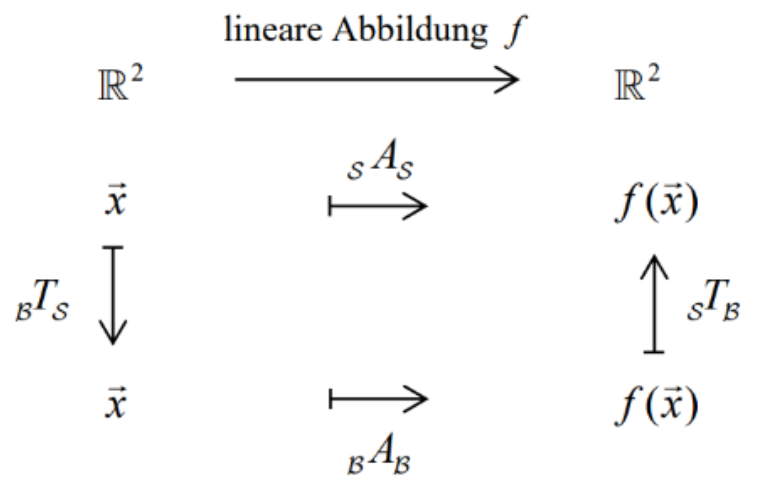
\includegraphics[width=0.6\textwidth]{koordinatentransformation.png}
    \end{center}
\end{concept}

\begin{example}
    $$
    B=\left\{\binom{2}{5}_{S} ;\binom{-1}{3}_{S}\right\}, \quad C=\left\{\binom{1}{0}_{S} ;\binom{1}{1}_{S} ;\binom{1}{2}_{S}\right\}
    $$
    $$
    { }_{C} T_{B}=\left(\begin{array}{cc}
    2 & -1 \\
    5 & 3
    \end{array}\right), \quad { }_{B} T_{C}=\left({ }_{C} T_{B}\right)^{-1}=\left(\begin{array}{cc}
    3 & 1 \\
    -5 & 2
    \end{array}\right)
    $$
\end{example}

\begin{KR}{Vollständiges Beispiel} 
    \\Kann mittels Inverse oder Gauss berechnet werden

    $$
    f: \mathbb{R}^{2} \rightarrow \mathbb{R}^{3}:\binom{x_{1}}{x_{2}} \rightarrow\begin{pmatrix} -x_{2} \\ 2 x_{1} \\ x_{2}-x_{1} \end{pmatrix}
    $$

    $$
    B=\left\{\binom{2}{5}_{S} ;\binom{-1}{3}_{S}\right\}, C=\left\{\begin{pmatrix} 1 \\ 0 \\ 1 \end{pmatrix}_{S} ;\begin{pmatrix} 0 \\ 2 \\ 1 \end{pmatrix}_{S} ;\begin{pmatrix} 1 \\ -4 \\ 1 \end{pmatrix}_{S}\right\}
    $$

    $$
    { }_{C} A_{B}={ }_{C}\left(\left(f\left(\frac{2}{5}\right)\right)_{C}\left(f\binom{-1}{3}\right)_{C}\right)_{B}
    $$

    \vspace{2mm}

    \resizebox{\textwidth}{!}{
    $
    \left(f \binom{2}{5}\right)_{C}=\begin{pmatrix} -5 \\ 4 \\ 3 \end{pmatrix}_{C}
    = \left(\begin{array}{ccc|c}
        1 & 0 & 1 & -5 \\
        0 & 2 & -4 & 4 \\
        1 & 1 & 1 & 3
        \end{array}\right)=\left(\begin{array}{ccc|c}
        1 & 0 & 0 & -11 \\
        0 & 1 & 0 & 14 \\
        0 & 0 & 1 & 6
        \end{array}\right)
    $}

    \vspace{2mm}

    \resizebox{\textwidth}{!}{
    $
    \left(f \binom{-1}{3}\right)_{C}=\begin{pmatrix} -3 \\ -2 \\ 4 \end{pmatrix}_{C}
    = \left(\begin{array}{ccc|c}
        1 & 0 & 1 & -3 \\
        0 & 2 & -4 & -2 \\
        1 & 1 & 1 & 4
        \end{array}\right)=\left(\begin{array}{ccc|c}
        1 & 0 & 0 & -11 \\
        0 & 1 & 0 & 15 \\
        0 & 0 & 1 & 8
        \end{array}\right)
    $}
    \vspace{2mm}
    
    $$
    { }_{C} A_{B}=\begin{pmatrix} -11 & -11 \\ 14 & 15 \\ 6 & 8 \end{pmatrix}_{B}
    $$
\end{KR}
